\section{Thiết kế luồng hoạt động}
Phần này trình bày các sơ đồ hoạt động mô tả những quy trình nghiệp vụ cốt lõi của hệ thống: nạp tài liệu, truy vấn RAG, và dọn dẹp dữ liệu. Các luồng này phản ánh cách hệ thống phối hợp giữa giao diện, máy chủ điều phối, PostgreSQL/\texttt{pgvector} và bộ định tuyến LLM. \cite{lewis2020retrieval,gao2023retrieval}

\subsection{Nạp và xử lý tài liệu}
Đây là quy trình khởi đầu, đóng vai trò quyết định đến chất lượng truy xuất của hệ thống RAG (UC-05, UC-07).

\begin{figure}[H]
    \centering
    \caption{Sơ đồ hoạt động của quy trình nạp và xử lý tài liệu}
    \label{fig:activity-ingest}
    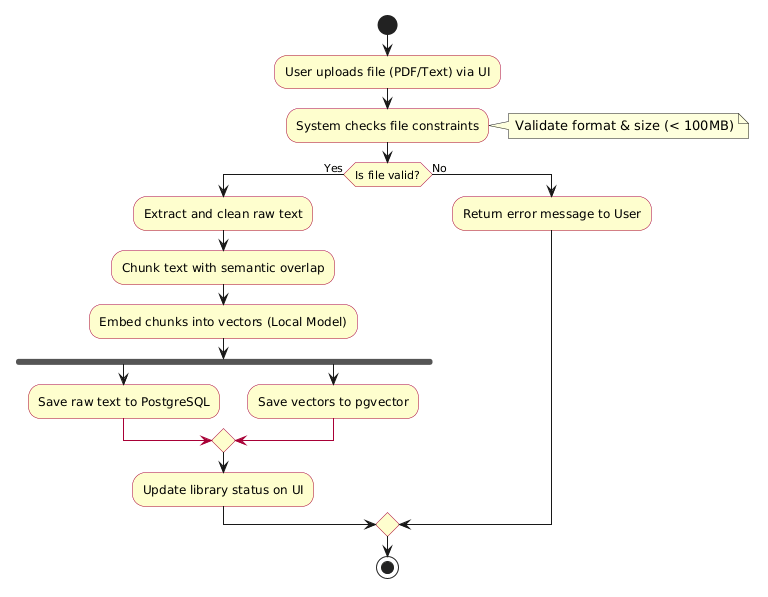
\includegraphics[width=0.92\linewidth]{images/activity-diagrams/ac-01.png}
\end{figure}

\begin{enumerate}
    \item Người dùng tải tệp PDF hoặc văn bản lên hệ thống thông qua giao diện.
    \item Máy chủ kiểm tra dung lượng, định dạng trước khi tiếp nhận tệp, lưu vào kho đối tượng và trả về ngay mã chấp nhận.
    \item Worker trích xuất văn bản thô; nếu không có lớp văn bản (PDF quét ảnh), worker chuyển sang luồng OCR (không thể hiện chi tiết trong sơ đồ trên, xem đặc tả UC-07).
    \item Văn bản được chia thành các đoạn nhỏ có chồng lấp để bảo toàn ngữ cảnh giữa các phân đoạn.
    \item Từng phân đoạn được chuyển qua mô hình nhúng cục bộ để tạo vector biểu diễn.
    \item Nội dung gốc và vector tương ứng được lưu đồng thời vào PostgreSQL với \texttt{pgvector}. \cite{reimers2019sentence,pgvector2023}
\end{enumerate}

\subsection{Truy vấn và phản hồi RAG}
Quy trình này mô tả cách hệ thống xử lý một câu hỏi để tạo phản hồi dựa trên ngữ cảnh tài liệu (UC-13, UC-14).

\begin{figure}[H]
    \centering
    \caption{Sơ đồ hoạt động của quy trình truy vấn và phản hồi RAG}
    \label{fig:activity-rag}
    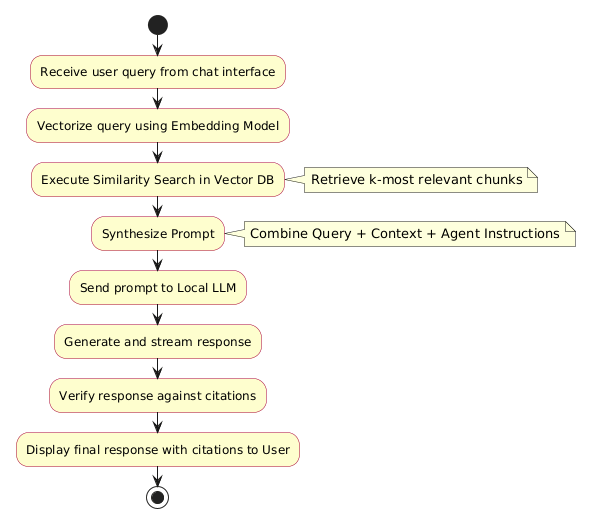
\includegraphics[width=0.88\linewidth]{images/activity-diagrams/ac-02.png}
\end{figure}

\begin{enumerate}
    \item Hệ thống tiếp nhận câu hỏi từ khung chat.
    \item Câu hỏi được nhúng hóa thành vector bằng cùng mô hình đã dùng ở giai đoạn lập chỉ mục.
    \item Hệ thống truy xuất các phân đoạn có độ liên quan cao nhất trong cơ sở dữ liệu vector.
    \item Câu hỏi, ngữ cảnh cứng (đoạn văn bản được chọn, nếu có) và ngữ cảnh truy xuất được ghép lại thành lời nhắc hoàn chỉnh cho bộ định tuyến LLM.
    \item Nhà cung cấp LLM khả dụng đầu tiên sinh phản hồi theo luồng (streaming).
    \item Hệ thống gửi trích dẫn nguồn kèm phản hồi cho giao diện hiển thị. \cite{lewis2020retrieval,gao2023retrieval}
\end{enumerate}

\subsection{Quản lý tài nguyên và dọn dẹp dữ liệu}
Quy trình này bảo đảm dữ liệu luôn nhất quán khi người dùng xóa tài liệu (UC-06).

\begin{figure}[H]
    \centering
    \caption{Sơ đồ hoạt động của quy trình quản lý tài nguyên và dọn dẹp dữ liệu}
    \label{fig:activity-cleanup}
    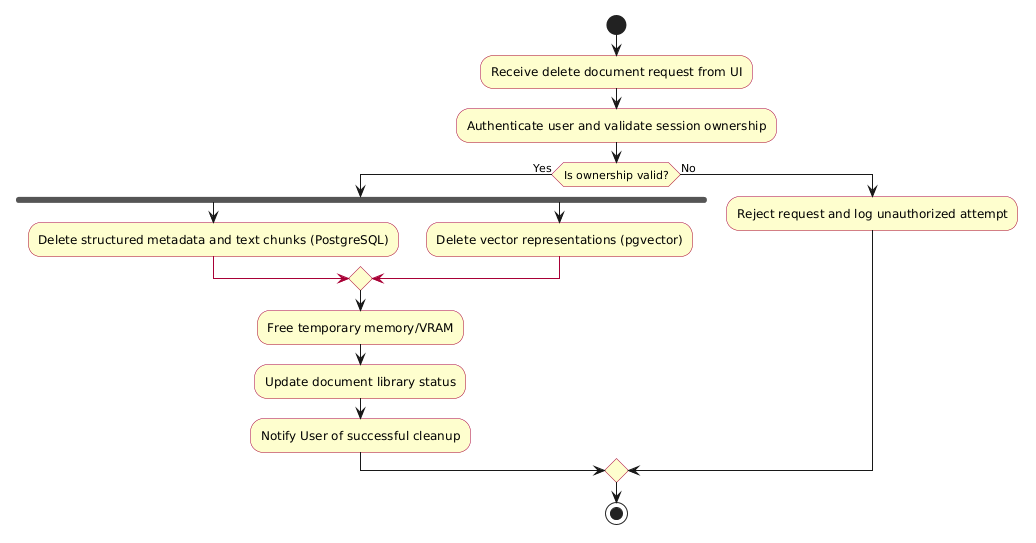
\includegraphics[width=0.96\linewidth]{images/activity-diagrams/ac-04.png}
\end{figure}

\begin{enumerate}
    \item Người dùng chọn hành động xóa tài liệu trong thư viện.
    \item Máy chủ kiểm tra quyền sở hữu (\texttt{user\_id}) trước khi thực hiện.
    \item Hệ thống xóa tệp vật lý khỏi kho lưu trữ đối tượng và phát lệnh xóa đến PostgreSQL.
    \item Cơ sở dữ liệu xóa tuần tự (cascade) các bản ghi liên quan: phân đoạn, vector, highlight và lịch sử hội thoại gắn với tài liệu.
    \item Giao diện cập nhật lại thư viện tài liệu sau khi quy trình hoàn tất. \cite{pgvector2023}
\end{enumerate}
